\section{Related Work}

The VGG architecture was introduced in \cite{KarenSimonyan.2014}. One of its key finings was to prefer deep CNNs (16-19 weight layers) with small receptive fields induced by using small kernels over shallow CNNs with bigger receptive fields. Therefore a configuration of 3x3 kernels with stride 1 were used. This not only helps to strengthen the discriminative character of the network as the non-linear activation function (ReLU) is applied more often but also keeps the number of parameters to train lower. To increase the non-linearity without affecting the related receptive fields even 1x1 kernels were considered in more deeper architectures. Only by using simple convolutional, max-pooling and fully connected layers at the end of the network, VGG achieved a 24.4 top-1 validation error score during ILSVRC-2014 (single net performance). \cite{KarenSimonyan.2014}

Regarding the top-5 test error score VGG got beaten by GoogLeNet with 6.67 compared to 7.32 from VGG. GoogLeNet uses a very deep CNN with 22 trainable layers with nine of them being the novel inception modules. To counter the higher computational costs that come with deeper architectures and also to prevent overfitting when having a limited dataset, an inception module uses 1x1 kernels for dimension reduction. To better recognize objects at various scales, an inception modules applies 1x1, 3x3 and 5x5 kernels simultaniously and bundles its results for the next layer making the network architecture also wider than others. \cite{ChristianSzegedy.2014}

When trying to answer the question how deep CNNs can get the so-called degradation problem was discovered. During training it was experienced that the loss curve started to ascent again once a specific depth threshold was passed. This was because once an ideal mapping to the right output vector was learned up until a certain depth by shallow layers, it was difficult to train the remaining layers to keep these values by learning an implicit identity function through several non-linearity steps. ResNet solved the degradation problem by introducing so-called shortcut connections that forward intermediate network values to deeper layers. The skipped network layers therefore only needed to learn the residual towards the expected output values giving ResNet its name. Therefore in case the optimal output is already learned, the weights of a residual component will turn to zero and an identity function is realized. Training an ensemble of 152 layer-deep ResNets on ImageNet as part of the ILSVRC-2015 challenge resulted in a 3.57 top-5 test error score beating both VGG and Inception from the previous challenge while keeping complexity eight times lower  than VGG for a single net. \cite{KaimingHe.2015}

The journey continues with DenseNet, a novel network architecture that feeds a layer all outputs from previous layers and passes its own feature maps towards all consecutive layers inside so-called dense blocks. It therefore makes feature propagation stronger by making feature reuse possible. Compared to ResNet, DenseNet achieves a lower error rate on CIFAR-10 with 4.51 to 6.61 at comparable depth while having less parameters to train. \cite{GaoHuang.2016}

A groundbreaking achievement was published with EfficientNets, a series of network architectures that were uniformly scaled in depth, width and resolution using a compound scaling method with fixed scaling coefficients for different hardware memory limits. 

\begin{figure}[t]
	\begin{center}
		% \fbox{\rule{0pt}{2in}\rule{0.9\linewidth}{0pt}}
		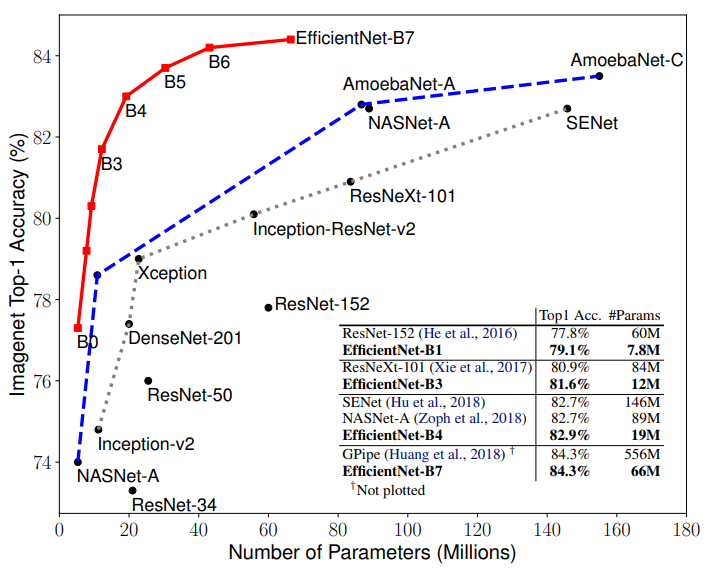
\includegraphics[width=0.8\linewidth]{images/efficientnet.PNG}
	\end{center}
	\caption{Comparison of EfficientNet to other state-of-the-art architectures on ImageNet (top-1 accuracy) compared to the number of parameters used}
	\label{fig:efficientnet}
\end{figure}

\autoref{fig:efficientnet} shows a 84.3\% top-1 accuracy score of EfficientNet-B7 on ImageNet outperforming other networks like ResNet or DenseNet while at the same time having far fewer parameters to train. \cite{LeMingxingTan.2019}

All these recent achievements on CNNs were based on manual architecture search. As opposed to such manual search, neural architecture search (NAS) tries to automate the process of finding suitable network architectures by iterating over a design space in a GridSearch-like manner. \cite{BarretZoph.2017}

One layer of abstraction higher, one can also search for suitable design spaces in order to derive a common understanding about important design principles. RegNet is such a design space derived from AnyNet, the largest possible design space without further constraints, by iteratively parametrizing whole populations of diverse networks and searching for the simplest but most perfomant population. Using this technique one can iteratively eliminate design space dimensions that are actually not too important for the network design because of similar perfomances. For instance, using a bootleneck compression ratio does not influence model performance and could thus be excluded from the design space by making it a static constraint. Increasing the depth or width of networks on the other hand is one of the key design space dimensions. The resulting population of RegNet was able to outperform EfficientNet. \cite{IlijaRadosavovic.2020}

-----------

- structural re-parameterization technique
- automatic, or manual architecture search